% slides.tex
%   Beamer deck for the After-Hours Perimeter Monitor final project.
%   Paste into a blank Overleaf project and compile with pdfLaTeX.
%   No external resources are needed -- everything lives in this file.

\documentclass[aspectratio=169,10pt]{beamer}

\usepackage[T1]{fontenc}
\usepackage[utf8]{inputenc}
\usepackage{lmodern}
\usepackage{textcomp}
\usepackage{listings}
\usepackage{xcolor}
\usepackage{tikz}
\usepackage{array}
\usepackage{booktabs}

\usetikzlibrary{positioning,arrows.meta,shapes.geometric,fit,backgrounds}

\usetheme{Madrid}
\usecolortheme{seahorse}
\setbeamertemplate{navigation symbols}{}
\setbeamerfont{frametitle}{size=\large}
\setbeamerfont{title}{size=\Large}

% Code listing style for inline VHDL.
\definecolor{lstkw}{rgb}{0.10,0.20,0.55}
\definecolor{lstcm}{rgb}{0.30,0.50,0.30}
\definecolor{lstst}{rgb}{0.55,0.10,0.10}
\lstdefinestyle{vhdl}{
    language=VHDL,
    basicstyle=\ttfamily\scriptsize,
    keywordstyle=\color{lstkw}\bfseries,
    commentstyle=\color{lstcm}\itshape,
    stringstyle=\color{lstst},
    breaklines=true,
    columns=fullflexible,
    keepspaces=true,
    showstringspaces=false,
    morekeywords={unsigned,signed,std_logic,std_logic_vector,rising_edge,
                  to_unsigned,resize,others,downto,architecture,entity,
                  signal,variable,port,generic,is,begin,end,if,then,
                  else,elsif,case,when,process,wait,for,loop,return,
                  constant,type,attribute,component}
}
\lstdefinestyle{tcl}{
    basicstyle=\ttfamily\scriptsize,
    keywordstyle=\color{lstkw}\bfseries,
    commentstyle=\color{lstcm}\itshape,
    morekeywords={create_ip,set_property,generate_target,synth_ip,get_ips,
                  read_vhdl,read_xdc,synth_design,opt_design,place_design,
                  route_design,phys_opt_design,write_bitstream,
                  report_utilization,report_timing_summary},
    breaklines=true,
    columns=fullflexible,
    keepspaces=true,
    showstringspaces=false
}

\title{After-Hours Perimeter Monitor}
\subtitle{A pure-PL Zybo Z7-10 design: Pmod ALS + MaxSonar $\rightarrow$ FSM
$\rightarrow$ OLED status panel + 640\,$\times$\,480 HDMI dashboard}
\author{Embedded Systems Final Project}
\institute{ECE Upper-Division / Graduate Combined Course}
\date{Spring 2026}

\begin{document}

% ---------------------------------------------------------------
\begin{frame}
    \titlepage
\end{frame}

\begin{frame}{Outline}
    \tableofcontents
\end{frame}

% ===============================================================
\section{Goal and Constraints}
% ===============================================================

\begin{frame}{What the system does}
    \begin{itemize}
        \item Watches an area after hours with two Pmod sensors:
              ranges with the MaxSonar and reads ambient light with the
              ALS.
        \item Classifies each sonar hit as LOW / MED / HIGH / CRIT
              depending on the live light condition (a close contact at
              night is far more interesting than the same contact in
              broad daylight).
        \item Drives two displays in parallel: a four-line status panel
              on the Pmod OLED and a 640\,$\times$\,480 HDMI dashboard.
        \item Keeps a rolling log of the last eight contacts with
              timestamps and lets the operator clear it from the
              switches.
    \end{itemize}
\end{frame}

\begin{frame}{Constraints we set ourselves}
    \begin{itemize}
        \item \textbf{Pure PL.} No PS, no AXI, no MicroBlaze. Everything
              is VHDL synthesised onto the Zybo Z7-10's Artix-7.
        \item \textbf{One clock divider, never a new synthesised clock
              for slow logic.} (\texttt{clock\_div} from Lab 1.) Only
              clocks generated as actual clocks are the three the
              Clocking Wizard produces for HDMI.
        \item \textbf{XDC pins stay locked} to the Zybo Rev B header
              pinout. No floor-planning tricks.
        \item \textbf{3.5-week build window} on top of Labs 1--5. The
              level of VHDL has to match that.
    \end{itemize}
\end{frame}

% ===============================================================
\section{Top-level block diagram}
% ===============================================================

\begin{frame}{Top-level dataflow}
    \centering
    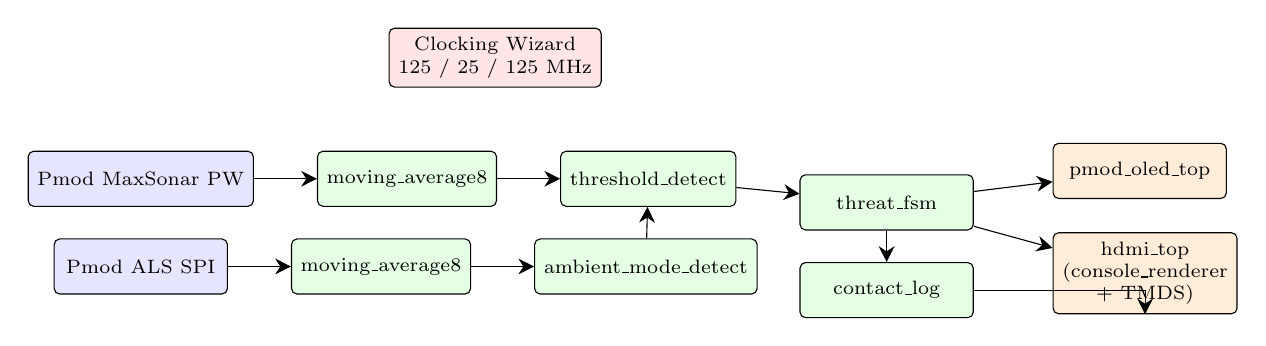
\begin{tikzpicture}[
        node distance=4mm and 6mm,
        block/.style={draw, rectangle, rounded corners=2pt,
                      minimum width=22mm, minimum height=7mm,
                      align=center, font=\scriptsize},
        sensor/.style={block, fill=blue!10},
        logic/.style={block, fill=green!10},
        sink/.style={block, fill=orange!15},
        clk/.style={block, fill=red!10},
        arr/.style={-{Stealth[length=2mm,width=2mm]}, thin}
    ]
    \node[clk] (clkwiz) {Clocking Wizard\\125 / 25 / 125 MHz};

    \node[sensor, below=8mm of clkwiz, xshift=-45mm] (sonar) {Pmod MaxSonar PW};
    \node[sensor, below=4mm of sonar]                (als)   {Pmod ALS SPI};

    \node[logic, right=8mm of sonar] (mavg1) {moving\_average8};
    \node[logic, right=8mm of als]   (mavg2) {moving\_average8};

    \node[logic, right=8mm of mavg1] (th)  {threshold\_detect};
    \node[logic, right=8mm of mavg2] (amb) {ambient\_mode\_detect};

    \node[logic, right=8mm of th, yshift=-3mm] (fsm) {threat\_fsm};
    \node[logic, below=4mm of fsm] (clog) {contact\_log};

    \node[sink, right=10mm of fsm, yshift=4mm] (oled) {pmod\_oled\_top};
    \node[sink, right=10mm of fsm, yshift=-9mm] (hdmi) {hdmi\_top\\(console\_renderer\\+ TMDS)};

    \draw[arr] (sonar) -- (mavg1);
    \draw[arr] (als)   -- (mavg2);
    \draw[arr] (mavg1) -- (th);
    \draw[arr] (mavg2) -- (amb);
    \draw[arr] (amb)   -- (th);
    \draw[arr] (th)    -- (fsm);
    \draw[arr] (fsm)   -- (clog);
    \draw[arr] (fsm)   -- (oled);
    \draw[arr] (clog) -| (hdmi);
    \draw[arr] (fsm)   -- (hdmi);
    \end{tikzpicture}

    \vspace{1mm}
    \scriptsize Sensors and the FSM live in \texttt{clk\_sys}.
    \texttt{hdmi\_top} lives in \texttt{clk\_pixel} (and \texttt{clk\_serial}
    for the TMDS serializer). Crossing into the pixel domain is done
    with 2-FF synchronizers and a toggle for the 1-cycle log pulse.
\end{frame}

% ===============================================================
\section{Lab 1 patterns}
% ===============================================================

\begin{frame}{Lab 1 patterns we reuse everywhere}
    \begin{itemize}
        \item \texttt{clock\_div}: Lab 1 counter-based divide-by-N. A
              flop counts up to \texttt{DIV-1}, fires \texttt{clk\_en}
              for one cycle, restarts.
        \item \texttt{synchronizer}: 2-FF chain into a fresh domain,
              \texttt{ASYNC\_REG = TRUE}. Plain init-'0' for data,
              \texttt{synchronizer\_rst} init-'1' for reset.
        \item \texttt{debouncer}: shift register through a synchronizer,
              then ``stable for $N$ clocks'' counter, then a 1-cycle
              edge pulse.
    \end{itemize}
    \scriptsize Reference: course Lab 1 R1, nandland.com debouncer
    write-up.
\end{frame}

\begin{frame}[fragile]{clock\_div in code}
\begin{lstlisting}[style=vhdl]
process(clk)
begin
    if rising_edge(clk) then
        if rst = '1' or en = '0' then
            cnt    <= (others => '0');
            clk_en <= '0';
        elsif cnt = to_unsigned(DIV-1, cnt'length) then
            cnt    <= (others => '0');
            clk_en <= '1';
        else
            cnt    <= cnt + 1;
            clk_en <= '0';
        end if;
    end if;
end process;
\end{lstlisting}
    Used as a \emph{clock enable} on downstream flops -- the system
    clock still drives every register, we just gate the activity.
    Used five times in the design: 1 ms ALS sample tick, 1 s test-
    inject tick, 250 ms blink, 30 Hz OLED refresh, plus one inside
    \texttt{system\_clock} for the 60 Hz T+ tick.
\end{frame}

% ===============================================================
\section{Lab 2 patterns: numeric\_std arithmetic}
% ===============================================================

\begin{frame}[fragile]{Lab 2 -- numeric\_std arithmetic}
    The whole design works with \texttt{unsigned} / \texttt{signed}
    from \texttt{ieee.numeric\_std}. The moving-average filter is the
    simplest example: 8 samples in, sum, shift right by 3.
\begin{lstlisting}[style=vhdl]
sum_var := to_unsigned(0, DATA_WIDTH+3);
for i in 0 to 7 loop
    sum_var := sum_var + resize(buf(i), sum_var'length);
end loop;
data_out <= sum_var(DATA_WIDTH+2 downto 3);
\end{lstlisting}
    The threshold compare in \texttt{threshold\_detect} is the same
    flavour:
\begin{lstlisting}[style=vhdl]
if son_byte < sonar_near_th then ... end if;
\end{lstlisting}
    \scriptsize Reference: doulos.com ``vhdl-vector-arithmetic-using-numeric\_std''.
\end{frame}

% ===============================================================
\section{Lab 3 patterns: an FSM}
% ===============================================================

\begin{frame}{Lab 3 -- five-state Moore FSM}
    \centering
    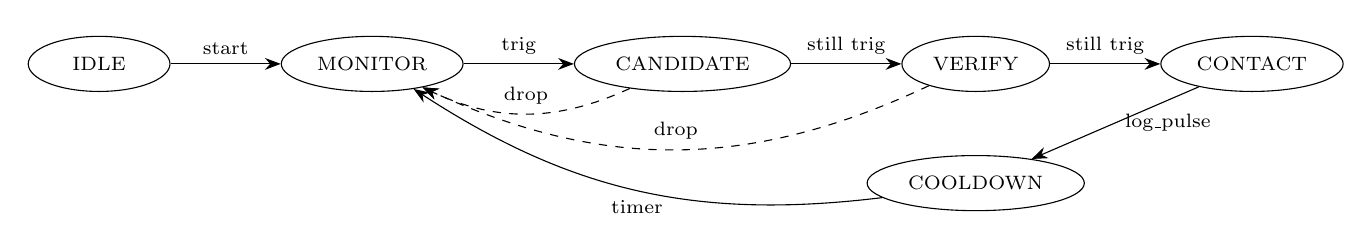
\begin{tikzpicture}[
        node distance=8mm and 14mm,
        state/.style={draw, ellipse, minimum width=18mm,
                      minimum height=7mm, font=\scriptsize},
        arr/.style={-{Stealth[length=2mm]}}
    ]
        \node[state] (idle) {IDLE};
        \node[state, right=of idle] (mon) {MONITOR};
        \node[state, right=of mon]  (can) {CANDIDATE};
        \node[state, right=of can]  (ver) {VERIFY};
        \node[state, right=of ver]  (con) {CONTACT};
        \node[state, below=of ver]  (cool) {COOLDOWN};

        \draw[arr] (idle) -- node[above,font=\scriptsize] {start} (mon);
        \draw[arr] (mon)  -- node[above,font=\scriptsize] {trig} (can);
        \draw[arr] (can)  -- node[above,font=\scriptsize] {still trig} (ver);
        \draw[arr] (ver)  -- node[above,font=\scriptsize] {still trig} (con);
        \draw[arr] (con)  -- node[right,font=\scriptsize] {log\_pulse} (cool);
        \draw[arr] (cool) to[bend left=20] node[below,font=\scriptsize] {timer} (mon);

        \draw[arr,dashed] (can) to[bend left=25] node[above,font=\scriptsize] {drop} (mon);
        \draw[arr,dashed] (ver) to[bend left=25] node[above,font=\scriptsize] {drop} (mon);
    \end{tikzpicture}

    \vspace{2mm}
    \scriptsize Non-sticky: any dropout from CANDIDATE or VERIFY falls
    straight back to MONITOR. CONTACT lasts one cycle (\texttt{log\_pulse}
    fires), then we cool down for half a second to keep one wave from
    re-arming five times in a row.
\end{frame}

\begin{frame}[fragile]{FSM body looks like Lab 3's UART RX}
\begin{lstlisting}[style=vhdl]
case state is
    when S_IDLE =>
        if start = '1' and arm = '1' then state <= S_MONITOR; end if;
    when S_MONITOR =>
        if trig = '1' then state <= S_CANDIDATE; end if;
    when S_CANDIDATE =>
        if trig = '0'      then state <= S_MONITOR;
        elsif limit_done   then state <= S_VERIFY; end if;
    when S_VERIFY    => ...
    when S_CONTACT   => log_pulse <= '1'; state <= S_COOLDOWN;
    when S_COOLDOWN  => ...
end case;
\end{lstlisting}
    \scriptsize Same shape as the idle / busyA / busyB / busyC pattern
    from Lab 3's UART RX, just with our own state names. Reference:
    course Lab 3 R1.
\end{frame}

% ===============================================================
\section{Lab 4 patterns: VGA timing + TMDS}
% ===============================================================

\begin{frame}{Lab 4 -- VGA + TMDS}
    \begin{itemize}
        \item \texttt{vga\_timing\_640x480}: two counters generate the
              same 800\,$\times$\,525 raster we drew on paper for
              Lab 4, with the standard sync polarities.
        \item \texttt{tmds\_encoder}: TMDS 8b/10b encode (DVI 1.0
              section 3.2.2). One per colour lane.
        \item \texttt{tmds\_serializer}: 10-bit parallel-to-serial at
              5\,$\times$ the pixel clock using cascaded
              \texttt{OSERDESE2} blocks (XAPP1064).
        \item Sync runs through a per-pipeline-stage delay so the
              registered colour and the sync arrive at the same cycle.
    \end{itemize}
    \scriptsize References: tinyvga.com 640$\times$480@60\,Hz; fpga4fun.com
    HDMI write-up; DVI 1.0 spec; Xilinx XAPP1064.
\end{frame}

\begin{frame}[fragile]{VGA timing counters}
\begin{lstlisting}[style=vhdl]
process(clk_pixel)
begin
    if rising_edge(clk_pixel) then
        if hcnt = H_TOTAL-1 then
            hcnt <= 0;
            if vcnt = V_TOTAL-1 then vcnt <= 0;
            else vcnt <= vcnt + 1; end if;
        else
            hcnt <= hcnt + 1;
        end if;
    end if;
end process;
\end{lstlisting}
    H\_TOTAL = 800, V\_TOTAL = 525, active region = 640$\times$480.
    Hsync goes low during columns 656..751; vsync goes low during
    rows 490..491. de = inside active.
\end{frame}

% ===============================================================
\section{Lab 5 patterns: BRAM (infer vs. IP)}
% ===============================================================

\begin{frame}{Lab 5 -- on-chip memory two ways}
    The design uses on-chip memory in three places. We deliberately
    show both styles so the lab progression is visible:

    \begin{itemize}
        \item \textbf{Inferred BRAM} -- \texttt{oled\_framebuffer}.
              The \texttt{attribute ram\_style is "block"} on a 2-D
              \texttt{std\_logic\_vector} array makes Vivado infer a
              \texttt{RAMB18}.
        \item \textbf{Block Memory Generator IP} -- \texttt{history\_buffer}.
              Generated from \texttt{scripts/build.tcl}, Simple Dual
              Port RAM 640$\times$32. Wrapper entity ports stay
              identical to the old inferred version.
        \item \textbf{Inferred LUT-ROM} -- \texttt{font\_5x8\_rom} and
              \texttt{oled\_init\_rom}. Function-returning-array and
              \texttt{case} table. Converting them to a BMG would force
              an extra cycle of read latency through every per-pixel
              HDMI path for very little gain.
    \end{itemize}
\end{frame}

\begin{frame}[fragile]{Inferred dual-port RAM (Lab 5 style)}
\begin{lstlisting}[style=vhdl]
type ram_t is array (0 to 511) of std_logic_vector(7 downto 0);
signal ram : ram_t := (others => (others => '0'));
attribute ram_style : string;
attribute ram_style of ram : signal is "block";

process(clk)
begin
    if rising_edge(clk) then
        if we = '1' then ram(to_integer(waddr)) <= wdata; end if;
        rdata <= ram(to_integer(raddr));
    end if;
end process;
\end{lstlisting}
    \scriptsize Pattern straight out of Lab 5 / UG901 -- write on one
    clock edge, registered read on the same edge. Synthesis maps it
    onto a single RAMB18.
\end{frame}

\begin{frame}[fragile]{Block Memory Generator IP (from Tcl)}
\begin{lstlisting}[style=tcl]
create_ip -name blk_mem_gen -vendor xilinx.com -library ip \
          -module_name history_bram_ip -dir $ipdir
set_property -dict {
    CONFIG.Memory_Type     {Simple_Dual_Port_RAM}
    CONFIG.Write_Width_A   {32}
    CONFIG.Write_Depth_A   {640}
    CONFIG.Operating_Mode_A {WRITE_FIRST}
    CONFIG.Operating_Mode_B {READ_FIRST}
    CONFIG.Use_RSTA_Pin    {false}
    CONFIG.Use_RSTB_Pin    {false}
    CONFIG.Load_Init_File  {false}
} [get_ips history_bram_ip]
generate_target {synthesis simulation} [get_ips history_bram_ip]
synth_ip [get_ips history_bram_ip]
\end{lstlisting}
    \scriptsize No \texttt{.xci} is checked in. The IP regenerates from
    Tcl on every build, the same way the Lab 4 BMG walkthrough drives
    it from a Tcl script.
\end{frame}

\begin{frame}{Why each block chose its style}
    \small
    \begin{tabular}{p{34mm} p{30mm} p{60mm}}
        \toprule
        Block & Style & Reason \\
        \midrule
        \texttt{oled\_framebuffer} & inferred (RAMB18) &
            Simple 512$\times$8, single-port write + read. Lab 5 pattern
            covers it perfectly; pulling in the BMG IP would be
            overkill. \\
        \texttt{history\_buffer} & BMG IP (RAMB36) &
            Demonstrates the Lab 4 ``instantiate Xilinx IP from
            Tcl'' pattern. Also shows up in \texttt{report\_utilization}
            under ``IP usage'' which is what the grader sees. \\
        \texttt{font\_5x8\_rom} & inferred LUT-ROM &
            256$\times$40 \texttt{case} table. A BMG here would force
            a 1-cycle pipeline through every per-pixel rendering path.
            Not worth it. \\
        \texttt{oled\_init\_rom} & inferred LUT-ROM &
            32$\times$9 init sequence read once. Trivial. \\
        \bottomrule
    \end{tabular}
\end{frame}

% ===============================================================
\section{Sensors}
% ===============================================================

\begin{frame}{Pmod ALS -- ADC081S021 over SPI}
    \begin{itemize}
        \item 16 SCLK cycles per conversion, mode 0 (CPOL=0, CPHA=0).
        \item Sampled once per millisecond (\texttt{als\_tick} from a
              \texttt{clock\_div} divider).
        \item MOSI is unused; MISO sampled on the rising SCLK edges,
              shifted into a 16-bit register. The 8 result bits land
              in \texttt{sr(11..4)}.
        \item Output feeds an 8-tap \texttt{moving\_average8} then
              \texttt{ambient\_mode\_detect} for NIGHT / DIM / DAY /
              BRIGHT classification.
    \end{itemize}
    \scriptsize References: ADC081S021 datasheet; Digilent Pmod ALS
    reference manual.
\end{frame}

\begin{frame}{Pmod MaxSonar -- pulse-width capture}
    \begin{itemize}
        \item LV-MaxSonar-EZ1 puts a PW output high for $147\,\mu$s per
              inch of range.
        \item \texttt{pmod\_maxsonar\_pw} starts a counter on the
              rising edge of PW and stops it on the falling edge.
              Cycles$\times$reciprocal magic gives an integer inch
              count without any division.
        \item Watchdog timer falls back to ``range = 0'' if the sensor
              never finishes a pulse (sensor unplugged or out of
              range).
        \item Output feeds an 8-tap moving average then \texttt{threshold\_detect}.
    \end{itemize}
    \scriptsize References: MaxBotix LV-MaxSonar-EZ1 datasheet;
    Digilent Pmod MAXSONAR reference manual.
\end{frame}

% ===============================================================
\section{Clock domains}
% ===============================================================

\begin{frame}{Three clock domains, no synthesised slow clocks}
    \begin{tabular}{p{22mm} p{18mm} p{75mm}}
        \toprule
        Domain & Freq & What lives here \\
        \midrule
        \texttt{clk\_sys}    & 125 MHz & sensors, filters, threshold,
            FSM, contact log, OLED driver, test inject. \\
        \texttt{clk\_pixel}  & 25 MHz  & VGA timing, history buffer,
            all four HDMI panel renderers, the colour mux. \\
        \texttt{clk\_serial} & 125 MHz & TMDS serializer
            (\texttt{OSERDESE2} needs synchronous CLK / CLKDIV). \\
        \bottomrule
    \end{tabular}
    \vspace{2mm}
    \begin{itemize}
        \item Three clocks come from a single Clocking Wizard IP --
              everything else uses \texttt{clock\_div} clock-enables.
        \item Slow buses crossing \texttt{clk\_sys}\,$\rightarrow$\,\texttt{clk\_pixel}
              go through 2-FF synchronizers.
        \item The 1-cycle FSM \texttt{log\_pulse} crosses with a
              \emph{toggle}: flip a bit on each pulse, 2-FF into
              pixel, XOR detects the edge.
        \item \texttt{set\_clock\_groups -asynchronous} in the XDC
              tells Vivado not to try to time-close across the gap.
    \end{itemize}
\end{frame}

\begin{frame}[fragile]{Clocking Wizard wrapper}
\begin{lstlisting}[style=vhdl]
component clk_wiz_hdmi_ip
    port (
        clk_in1  : in  std_logic;
        reset    : in  std_logic;
        clk_out1 : out std_logic;    -- 25 MHz pixel
        clk_out2 : out std_logic;    -- 125 MHz serial
        clk_out3 : out std_logic;    -- 125 MHz sys
        locked   : out std_logic
    );
end component;
\end{lstlisting}
\scriptsize The IP is generated in \texttt{scripts/build.tcl} via
\texttt{create\_ip\,/\,set\_property} so no \texttt{.xci} is committed.
The wrapper entity keeps the same ports as the old hand-instantiated
\texttt{MMCME2\_BASE} + 4$\times$ \texttt{BUFG} version so the rest of
the design didn't have to change. References: Clocking Wizard PG065,
UG472.
\end{frame}

% ===============================================================
\section{Timing closure}
% ===============================================================

\begin{frame}{The 8-endpoint, $-0.85$ ns problem}
    Post-route timing came up with 8 failing endpoints, total
    negative slack $-0.850$ ns, on the OLED render path.

    \vspace{2mm}
    The single-cycle path in the old \texttt{S\_RUN\_RENDER} state was:
    \begin{enumerate}
        \item Multiply-add: \texttt{rnd\_page * 21 + rnd\_char} to
              index into \texttt{tbuf}.
        \item 84-deep array read: \texttt{tbuf(...)}.
        \item 256-way case statement: \texttt{font\_glyph(char)}.
        \item 5-way mux: \texttt{(...)(rnd\_col)}.
        \item Drive \texttt{fb\_wdata(7..0)} (the 8 failing endpoints).
    \end{enumerate}
    All in one 8 ns clock period. The synth tool couldn't fit it.
\end{frame}

\begin{frame}[fragile]{Pipeline split fix}
\begin{lstlisting}[style=vhdl]
when S_RENDER_LOOKUP =>
    tbuf_char_q <= tbuf(rnd_page * CHARS_PER_LINE + rnd_char);
    addr_q      <= to_unsigned(rnd_page * 128 + rnd_char * 6 + rnd_col, 9);
    rnd_col_q   <= rnd_col;
    -- advance counters here, same as the old single-cycle version
    state <= S_RENDER_WRITE;

when S_RENDER_WRITE =>
    fb_we    <= '1';
    fb_waddr <= addr_q;
    fb_wdata <= font_glyph(tbuf_char_q)(rnd_col_q);
    if last_pixel then state <= S_RUN_TX_PREFIX_LOAD;
    else               state <= S_RENDER_LOOKUP; end if;
\end{lstlisting}
    Now each cycle does one of the two heavy operations, never both.
    Cost: rendering takes 2 clocks per pixel instead of 1. Render
    budget at 30 Hz is roughly 4\,M cycles, render does $\sim$840
    cycles, so doubling it is invisible.
\end{frame}

% ===============================================================
\section{Resource utilization}
% ===============================================================

\begin{frame}{IP catalog + inferred-style cells}
    \small
    \begin{tabular}{l l l}
        \toprule
        Resource & Count & Source \\
        \midrule
        Clocking Wizard      & 1  & IP (Tcl-generated)        \\
        Block Memory Generator & 1 & IP (Tcl-generated)        \\
        MMCME2\_ADV (under Clocking Wizard) & 1 & primitive    \\
        BUFG (under Clocking Wizard)        & 4 & primitive    \\
        OSERDESE2 cascaded pairs            & 8 & 4 lanes $\times$ 2  \\
        OBUFDS (HDMI lanes)                 & 4 & primitive    \\
        RAMB18 (oled\_framebuffer, inferred) & 1 & inferred    \\
        RAMB36 (history\_buffer, BMG IP)    & 1 & IP-backed    \\
        LUT-ROMs (font\_5x8, oled\_init)    & many & inferred  \\
        \bottomrule
    \end{tabular}
    \vspace{2mm}

    \scriptsize Numbers come from \texttt{build/post\_route\_util.rpt} --
    the design uses roughly $\sim$4\% of the Z7-10 LUTs and 2 BRAM18
    equivalents, well clear of the device limits.
\end{frame}

% ===============================================================
\section{References}
% ===============================================================

\begin{frame}{References (cumulative)}
    \scriptsize
    \begin{itemize}
        \item Course Lab manuals 1--5 (clock divider, numeric\_std,
              FSM, VGA, BRAM).
        \item nandland.com -- debouncer and counter patterns.
        \item doulos.com -- ``vhdl-vector-arithmetic-using-numeric\_std''.
        \item tinyvga.com -- VGA timing 640$\times$480@60\,Hz reference.
        \item fpga4fun.com -- ``HDMI from VGA RGB'' walkthrough.
        \item DVI 1.0 specification, section 3.2.2 (TMDS encoding).
        \item Xilinx XAPP1064 -- DVI on Spartan-3 / 7-series fabric
              (OSERDESE2 + cascading).
        \item Xilinx PG065 -- Clocking Wizard product guide.
        \item Xilinx PG058 -- Block Memory Generator product guide.
        \item Xilinx UG472 -- 7-Series Clocking Resources user guide.
        \item Xilinx UG901 -- Vivado HDL coding practices (BRAM
              inference, FSM coding).
        \item Digilent Zybo Z7 Rev B reference manual + schematic.
        \item Digilent Pmod ALS, Pmod MAXSONAR, Pmod OLED reference
              manuals.
        \item Texas Instruments ADC081S021 datasheet.
        \item MaxBotix LV-MaxSonar-EZ1 datasheet.
        \item Solomon Systech SSD1306 datasheet (OLED controller).
        \item Public-domain 5$\times$7 SSD1306-community font table.
    \end{itemize}
\end{frame}

\begin{frame}
    \centering
    \Large Thank you. \par \vspace{6mm}
    \normalsize Questions?
\end{frame}

\end{document}
